\documentclass[a4paper,pt12]{article}
\usepackage{graphicx}
\usepackage{url}
\usepackage{placeins}

\begin{document}
\author{Pascal Stammer, Mats Richter, Benjamin Henne}
\title{Final Project: A Comparison Of Siamese Oneshot Classification With Softmax Classification using Deep Neural Networks}


\maketitle

\begin{abstract}
Learning from Dataset with sparse samples for individual classes and high inbalance in the distribution of classes is a big issue in deep learning and machine learning in general. Modern deep learning architectures usally require thousands of data points per class to learn generalizing concepts. Siamese Networks are an attempt to create a classifier that is very robust towards class inbalances and (in theory) able to distinguish classes by only seeing a single sample of one of the two classes (oneshot classification). This work evaluates the classification performance of a siamese neural network by comparing the classification performance against a very similar, softmax-classification convolutional neural network. We will compare the baseline performance differences between the network on a balanced dataset and further compare the performance on highly inbalanced data. 

\end{abstract}

\section{Introduction}

\subsection{Siamese Neural Networks}

\section{Experiments}
The experiments are aimed to look into the differences in learning behaviour between deep neural networks and siamese deep neural networks. We therefore used two simple and very similar showcase  architectures to make this comparison as clear as possible. We used the MNIST and the quantiatively larger EMNIST datasets as our data basis for our experiments. We altered the datasets class balance and the number of classes to compare the performance of both networks in increasingly difficult situations with regards to the structure of the dataset while keeping the data itself relatively simple.  

\subsection{Network Architectures}
In order to make the performance of both networks comparable and keep the complexity of the models as simple as possible, both architectures are only diverging by it's siamnese property. We also refused to use more complex architectural features like highway connections or multiple paths like in the Inception architectures, to rule out more complex influences on the typical learning behaviour of convolutional neural networks.

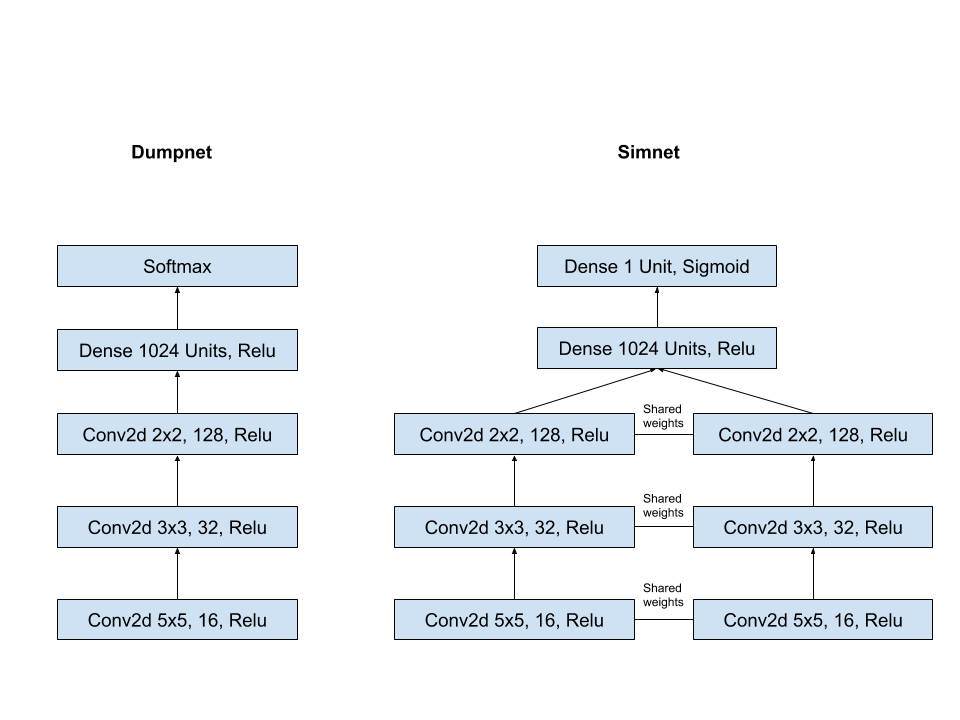
\includegraphics[scale=0.3]{nets.png}

\subsubsection{Dumbnet}
This network is our baseline model for comparing and evaluating the performance of the siamese network.  It consists of 3 convolutional layer with relu activation functions, valid padding, and increasing filter size. \newline
The output of the convolutional part (from now on called stem) of the network is read out by a single dense layer with 1024 units and relu activation function and fed into a 10 way (MNIST) or 62 way (EMNIST) softmax. For optimization a Adam Optimizer with default parameters was used.

\subsubsection{Simnet}
Simnet is derived from the Dumbnet architecture. The siamese part consists of two steam, each identical to the one of dumpnet. Each stem receives a single image as input. The readout is concatenated and put into a dense layer with 1024 units with relu activation function and a single unit output with sigmoidal activation function. \newline
Simnet is trained by randomly aranging the images into pairs. The labels are created like in \cite{siamese}, non matching original labels result in 1, matching original labels result in 0. This process is repeated for each epoch of training. \newline
The loss of the network is weighted by $1:10$ (MNIST) or $1:62$ (EMNIST) in favour of matching original labels, since due to the statistical probability of two random images belonging to the same class. This implies the assumption of balanced classes, even though the EMNIST dataset is not balanced. This is intentional, since no sample or class weights are applied on the loss of Dumpnet, which implies also the assumption of balanced classes. \newline
A normal Gradient Decent optimizer was used, since Adam lead to instabilities in the learning dynamics. The default values were kept the same.

\subsection{Data and Experimental Setups}

\subsubsection{MNIST Experiments}
The MNIST dataset is one of the quasi standard datasets in machine learning and deep learning. It is a balanced dataset consisting of binary, square images with a size of 28 pixels on each side. There are ten classes resembling handwritten digits from zero to nine. The dataset is balanced and known to be very solveable for simple computer vision algorithms with little noise and no missclassifications in the ground truth. \newline
The MNIST performance serves as baseline of performance on a sovable, balanced classification problem. 

\subsubsection{EMNIST Experiments}
EMNIST is a novel extension for the MNIST dataset. We used the by-class version of the dataset with 62 classes, containing additional classes for handwritten letters (lower and capital are treated as seperate classes). The most important property of this dataset is the relatively close resemblance to MNIST by simultaniousny beeing a more complex classification problem with strong inbalances between the classes.

\section{Results}

\subsubsection{MNIST Experiments}

\subsubsection{EMNIST Experiments}

\section{Conclusion}


% Dieser Stil erzeugt Verweise mit Autorenname und Jahr
%\bibliographystyle{gerapali}
%\bibliographystyle{wmaainf}
\bibliographystyle{plain}
\addcontentsline{toc}{chapter}{Literaturverzeichnis}

% Hier die Datei (ohne .bib) angeben, in der die referenzierten
% Paper stehen
\nocite{*}
\bibliography{literatur}
\end{document}